
%%%%%%%%%%%%%%%%%%%%%%%%%%%%%%%%%%%%%%%%%%%%%%%%%%%%%%%%%%%%%%%%%%%%%%%%
%Para las ecuaciones siempre es Ec.(n).
%Para las figuras siempre es Fig.n, incluso en el caption de la figura. Tambien las Tablas
%Para las referencias es [n]
%%%%%%%%%%%%%%%%%%%%%%%%%%%%%%%%%%%%%%%%%%%%%%%%%%%%%%%%%%%%%%%%%%%%%%%%

\documentclass[
reprint,
%notitlepage,
%superscriptaddress,
%groupedaddress,
%unsortedaddress,
%runinaddress,
%frontmatterverbose, 
%preprint,
%showpacs,preprintnumbers,
%nofootinbib,
%nobibnotes,
%bibnotes,
%11 pt,
amsmath,
amssymb,
aps,
%pra,
%prb,
%rmp,
%tightenlines %esto hizo el milagro de sacar los espacios en blancos estocásticos (?)
 %prstab,
%prstper,
%floatfix,\textbf{}
]{revtex4-1} %Instalar primero para usarlo. Paquete malo.

%\documentclass[onecolumn, aps, amsmath,amssymb ]{article}
\usepackage{lipsum}  
\usepackage{graphicx}% Include figure files
\usepackage{subfig}
\usepackage{braket}
\usepackage{comment} %comment large chunks of text
\usepackage{dcolumn}% Align table columns on decimal point
\usepackage{bm}% bold math
%\usepackage{hyperref}% add hypertext capabilities
\usepackage[mathlines]{lineno}% Enable numbering of text and display math
%\linenumbers\relax % Commence numbering lines
\usepackage{mathtools} %% Para el supraíndice

\usepackage[nice]{nicefrac}

%%%%%%%El Señor Español%%%%%%%%%%%%%%%%%%%%%%%%%%%
\usepackage[utf8]{inputenc} %acento
\usepackage[
spanish, %El lenguaje.
es-tabla, %La tabla y no cuadro.
activeacute, %El acento.
es-nodecimaldot %Punto y no coma con separador de números
]{babel}
\usepackage{microtype} %para hacerlo más bonito :33 como vos (?) 
%%%%%%%%%%%%%%%%%%%%%%%%%%%%%%%%%%%%%%%%%%%%%%%%%%%
%%%%%%%%% Para que las imágenes se queden dónde las quiero (?
\usepackage{float}
%%%%%%%%%%

%%%%%%%%Cambia a Fig de Figure%%%%%%%%%%
\makeatletter
\renewcommand{\fnum@figure}{Fig. \thefigure} 
\makeatother
%%%%%%%%%%%%%%%%%%%%%%%%%%%%%%%%%%%%%%%%
\raggedbottom


\begin{document}
%%%%%%%%%%%%%%%%%%%%%%%%%%%%%%%%%%Título%%%%%%%%%%%%%%%%%%%%%%%%%%%%%%%%%%%%%%
%%%%%%%%%%%%%%%%%%%%%%%%%%%%%%%%%%%%%%%%%%%%%%%%%%%%%%%%%%%%%%%%%%%%%%%%%%%%%%

\title{Anisotropías para todos los disparos y pesos de los hexágonos}
\author{Evelyn~G.~Coronel}

\affiliation{
Tesis de Maestría en Ciencias Físicas\\ Instituto Balseiro\\}

\date[]{\lowercase{\today}} %%lw para lw, [] sin date

%\begin{abstract}

%\end{abstract} 
\maketitle
%%%%%%%%%%%%%%%%%%%%%%%%%%%%%%%%%%%%%%%%%%%%%%%%%%%%%%%%%%%%%%%%%%%%%%%%%%%%%%%%%%%
% Podemos usar cualquiera de los dos comandos: \input o \include para incluir el texto

%\subsubsection{Nomenclatura}
%ai
%	\begin{table}[H]
%	\centering
%		\begin{tabular}{c|c|c|c}
%	Archivo AllTriggers  & \text{Eventos} & UTC inicial &  UTC final  \\ \hlineaiai
%	2020			 & 13 739 351	  &  1372680068	&  1577879983 \\ %2019
%	2019			 & 	8 463 063	  &	 1372680068 &  1496318388 \\ %Herald
%	2017			 &	8 592 302	  &  1372680068 &  1498521517 \\ %Oscar
%			\end{tabular}
%			\end{table}
%



\section{Anisotropías  considerando el peso de los hexágonos}

\subsection{Verificando que todo funcione como debe}


%Efectos espúreos: Por un lado estan esos piquitos chiquitos, que parecen ser algun problema numerico. Por otro hay todavia demasiados picos arriba de la linea de 99%.


%Se me ocurren dos checks que podrias hacer:

\subsubsection{Comparando con los datos de Oscar}
% 	1-  Uno, que tal vez ya hiciste, es correr tu programa en los datos que uso Oscar y ver de repetir los plots para las dos energias arriba de full efficiency (4-8 y >8)  para ver que el programa funciona igual

\begin{itemize}
	\item Agregar figuras sin peso 
	\begin{itemize}
		\item El de 4-8 para el 2017
		\item >8 para el 2017
	\end{itemize}
	\item buscar los valores de los dipolos conocidos y compararlos con lo que obtengo (usando los pesos)
\end{itemize}

\subsubsection{¿Análisis en frecuencia de los hexágonos?} \label{analisis_peso}
% 	2- Otra prueba que podrias hacer es hacer un  analisis en frecuencia  similar al que hiciste pero para la modulacion de hexagonos sola. Esto seria para ver que no hay cosas raras en el rate de hexagonos de estos datos. No tengo del todo claro como se haria. En vez de hacer la suma de senos y cosenos en los tiempos del zenit cuando llega un evento como ahora, habria que hacer esas sumas en un espaciado constante de tiempo (podrian ser los 5' en que estan bineados, y los pesos deberian ser proporcional a la cantidad de hexagonos. Pensalo un poco como se podria implementar y si queres lo charlamos despues.
\begin{itemize}
	\item ¿Barrido en frecuencia en ascensión recta?
	\item ¿Barriendo el archivo de eventos pero en vez de usar el evento para analizar, uso el valor del peso para el bin correspondiente? Suena bien.
\end{itemize}


%Hola, la fig 1 tiene en solar algunos saltos un poco raros. Podrias hacer esa misma figura (hexagonos en  solar, sidereo y antisidereo) para el periodo de tiempo desde 2004 a dic 2017 (asi comparamos con la comparacion que habian hecho Oscar y Ugo hace un tiempo.
%Y tambien hacela para el periodo completo hasta dic 2019, asi vemos lo que se usa para la ultima parte de tu documento.

\subsubsection{Comparando los pesos en sidérea, solar y antisiderea.}

Un ejemplo de como son los pesos para tres frecuencias en particular, para el rango 2013-2019, se muestra en la Fig.\,\ref{fig:pesos}


\begin{figure}[H]
	\centering
	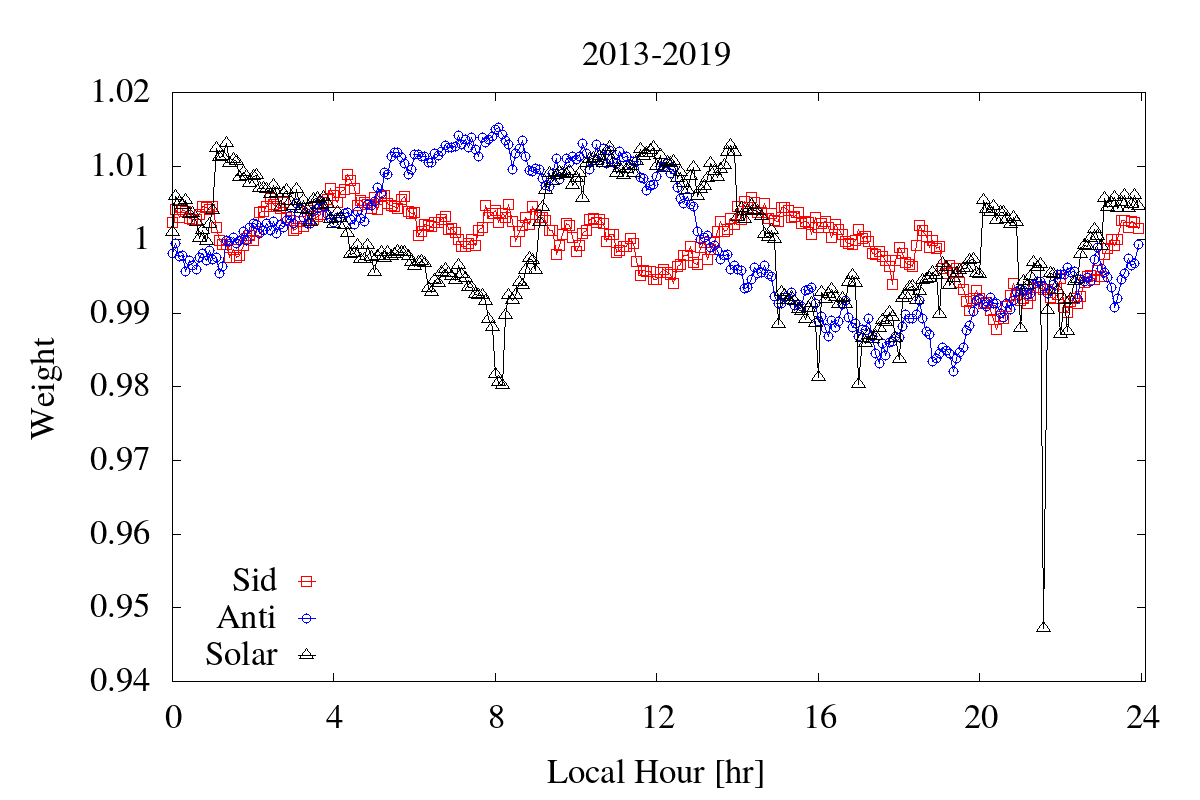
\includegraphics[width=0.5\textwidth]{Graficos/weigth2013-2019.png}
	\caption{Pesos para las frecuencias sidérea, solar y anti-sidérea en el rango 2013-2019}
	\label{fig:pesos}
\end{figure}


Para el rango del 2004 hasta Jun 2017

\begin{figure}[H]
	\centering
	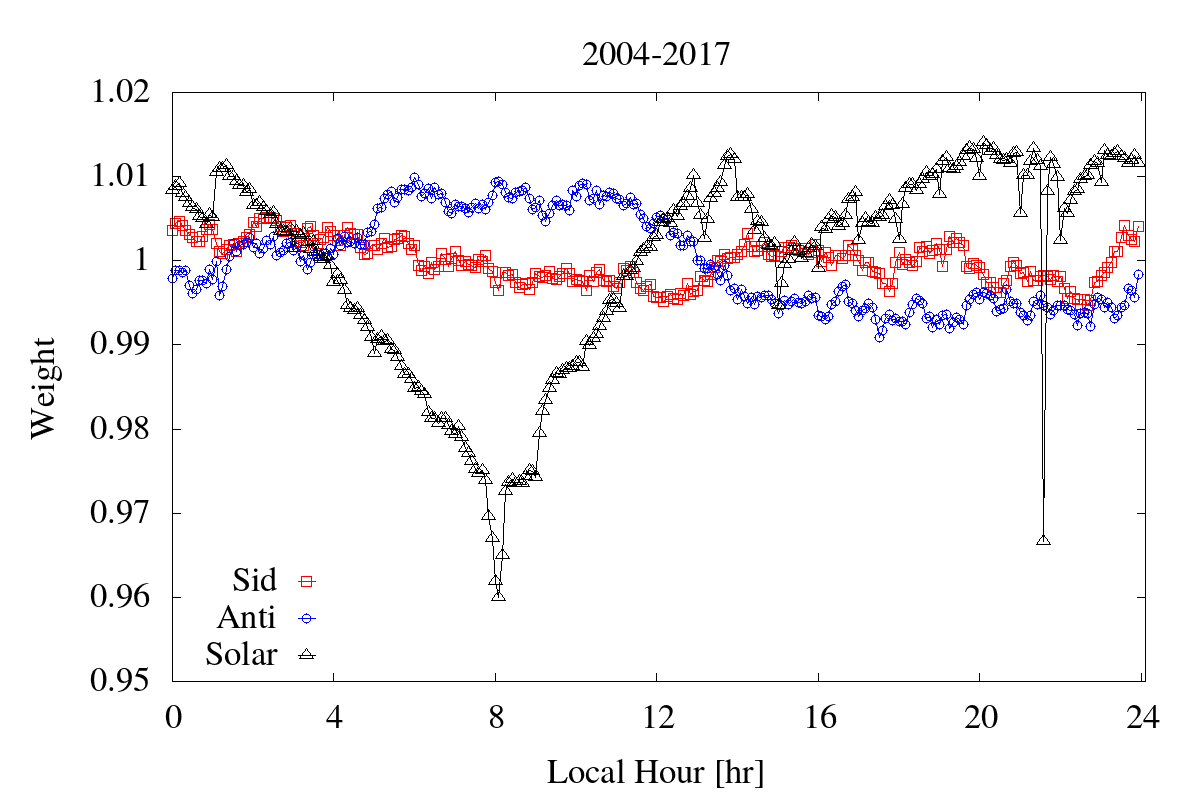
\includegraphics[width=0.5\textwidth]{Graficos/weigth2004-2017.png}
	\caption{Pesos para las frecuencias sidérea, solar y anti-sidérea en el rango 2004-2017}
	\label{fig:pesos_2017}
\end{figure}



Para el rango entre el $2005$ y $2019$
\begin{figure}[H]
	\centering
	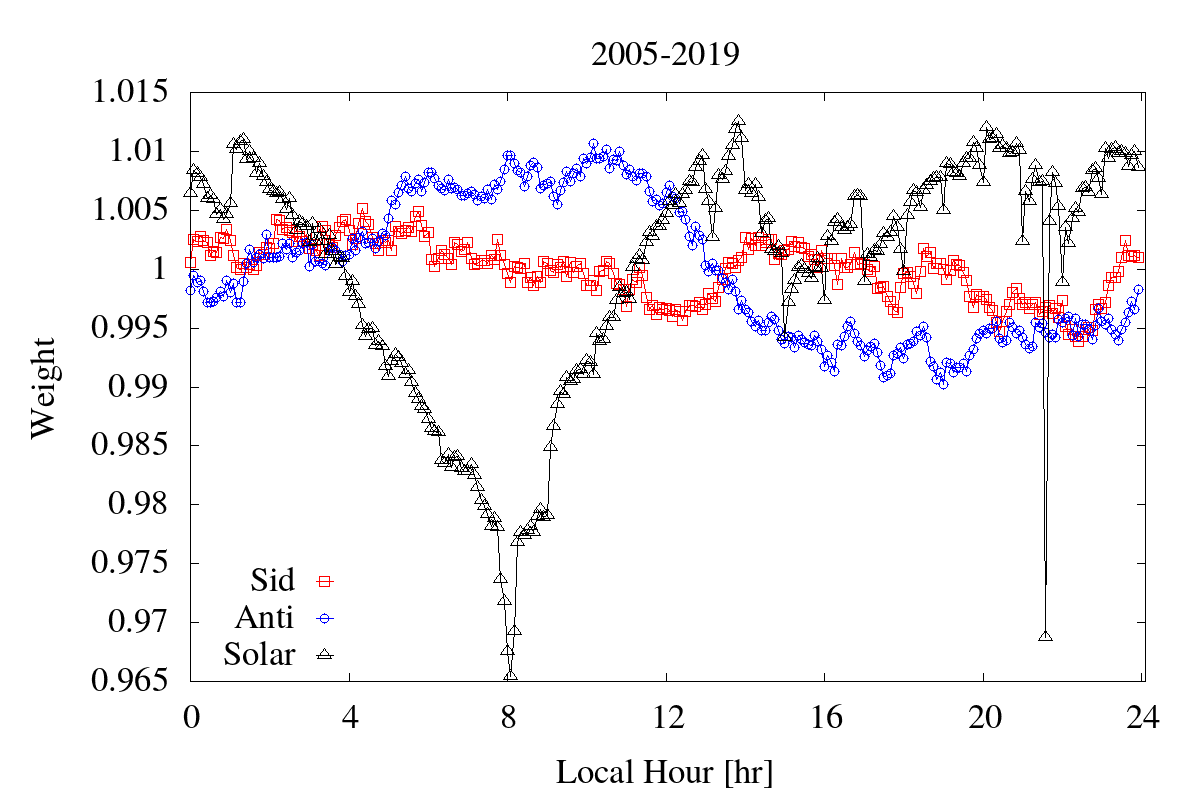
\includegraphics[width=0.5\textwidth]{Graficos/weigth2005-2019.png}
	\caption{Pesos para las frecuencias sidérea, solar y anti-sidérea en el rango 2005-2019}
	\label{fig:pesos_2019}
\end{figure}




La idea que tengo sobre el pico en ambos gráficos es algo en la cantidad de hexagonos, algún periodo donde se apagó la mitad del observatorio o algo así. Quiero hacer la evolución de la cantidad de hexagonos para ese bin en particular en la frecuencia. Estaba pensando en como codearlo para que me sirva también para hacer \ref{analisis_peso}.


%Otra cosa, en general: seria bueno hacer los plots entre 363.25 y 367.25 (ya que las tres que nos interesan son 364.25, 365.25 y 366.25). PARA DESPUÉS
%Otra curiosidad, en frecuencia siderea, cual es la fase en RA y la probabilidad del bin entre 1y 2?


\subsection{Variación de los pesos en función de la ascensión recta}
En las figuras de esta sección se muestran el análisis en ascensión recta para los eventos de observatorio considerando las variaciones de la exposición. 
Los mismos se hicieron en el mismo intervalo de tiempo para poder compararlos entre sí. Elegí el rango presentado en la Tabla \ref{rango_corto}  porque en el mismo se encuentran todos los eventos filtrados por energía, por bad period, por reconstrucción correcta, etc. El rango empieza en el 2013 porque la última versión del archivo de todos los disparos empezó a registrarse desde el  1 de Julio del 2013 a las 12:01:08 GMT (1372680068) hasta el  1 de enero del 2020 a las 11:59:43 (1577879983). Mientras que el archivo del disparo estándar va desde el 01 de enero del 2004.

	\begin{table}[H]
	\centering
		\begin{tabular}{c|c|c|c}
	 		& UTC 			& Fecha		 	&  Hora GMT  \\ \hline
	Inicio	& 1372699409	&2013-07-01 	&17:23:29		\\
	Final 	& 1577825634	&2019-12-31 	&20:53:54		\\
		\end{tabular}
	\caption{Rango de tiempo considerando todos los disparos} 	\label{rango_corto}
	\end{table}


\subsubsection{Energía entre 1\,EeV y 2\,EeV}

Para este caso utilizamos el archivo con todos los disparos en el rango de energía $1\,$ EeV - $2\,$EeV donde se tiene $1\,321\,702$ eventos.

\begin{figure}[H]
	\centering
	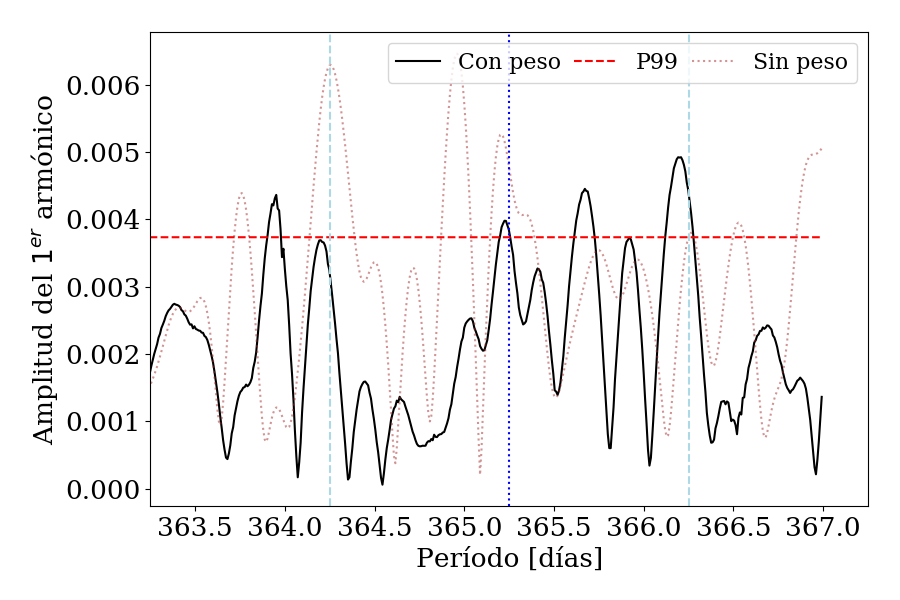
\includegraphics[width=0.5\textwidth]{Graficos/2019_AllTriggers_1_2_EeV_con_vs_sin_peso.png}
	\caption{Todos los disparos: entre 1 EeV y 2 EeV, entre 2013-2019}
	\label{fig:12w}
\end{figure}
%fig

\emph{Otra curiosidad, en frecuencia siderea (366.25), cual es la fase en RA y la probabilidad del bin entre 1y 2?}

La siguiente tabla se había calculado usando la formula 

\begin{equation}
	\tilde \alpha = 2\pi \frac{t_i}{T_x} +\alpha_i - \alpha^0
\end{equation}
donde $\alpha_i$ y $\alpha^o$ con las RA del evento y del cenit del observatorio.

	\begin{table}[H]
	\centering
		\begin{tabular}{c|c}
	 		&  2013-2019 (Con peso)	 \\ \hline
	Fase		& 	306.611				 \\
	$r$ 		&  0.00440897			\\
	$r_{99}$ 	&  0.00373348			\\
	$P(\tilde r)$ 	    & 	0.162485	\%	 \\
		\end{tabular}
	\caption{Rango de tiempo considerando todos los disparos} 	\label{rango_corto}
	\end{table}


\subsubsection{Energía entre 2\,EeV y 4\,EeV}

Para este caso utilizamos los eventos del archivo con todos los disparos con energía entre $2\,$ EeV - $4\,$EeV, donde se encontraron $288\,444$ eventos.
\begin{figure}[H]
	\centering
	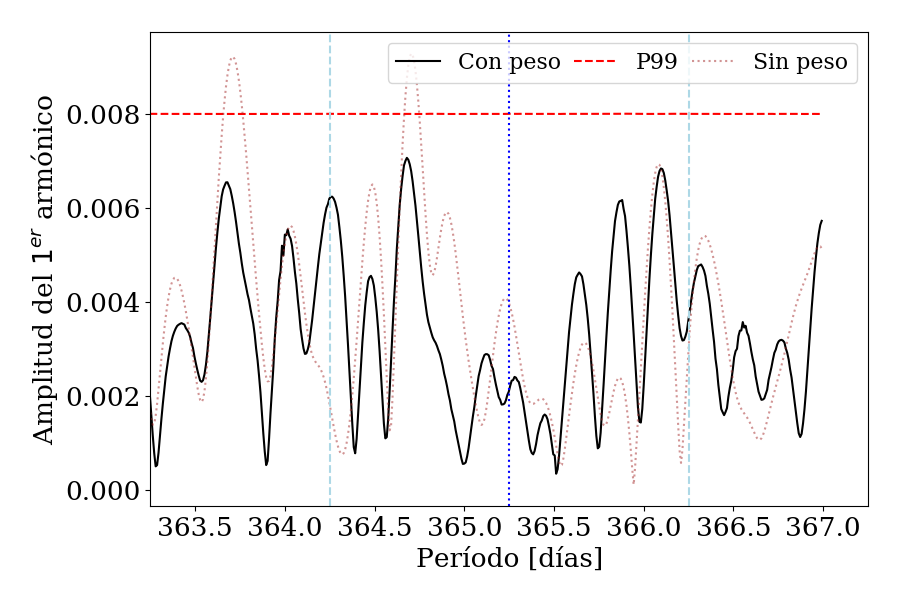
\includegraphics[width=0.5\textwidth]{Graficos/2019_AllTriggers_2_4_EeV_con_vs_sin_peso.png}
	\caption{Todos los disparos: entre 2 EeV y 4 EeV, entre 2013-2019}
	\label{fig:24w}
\end{figure}

En la Fig.\,\ref{fig:24w} no se ve ningún pico por encima de  percentil 99.


\subsubsection{Energía entre 4\,EeV y 8\,EeV}

A partir de $3\,$EeV el disparo estándar tiene una eficiencia del $100\%$. Entonces para este  intervalo de energías,  utilizamos el archivo con el disparo estandar.

\begin{figure}[H]
	\centering
	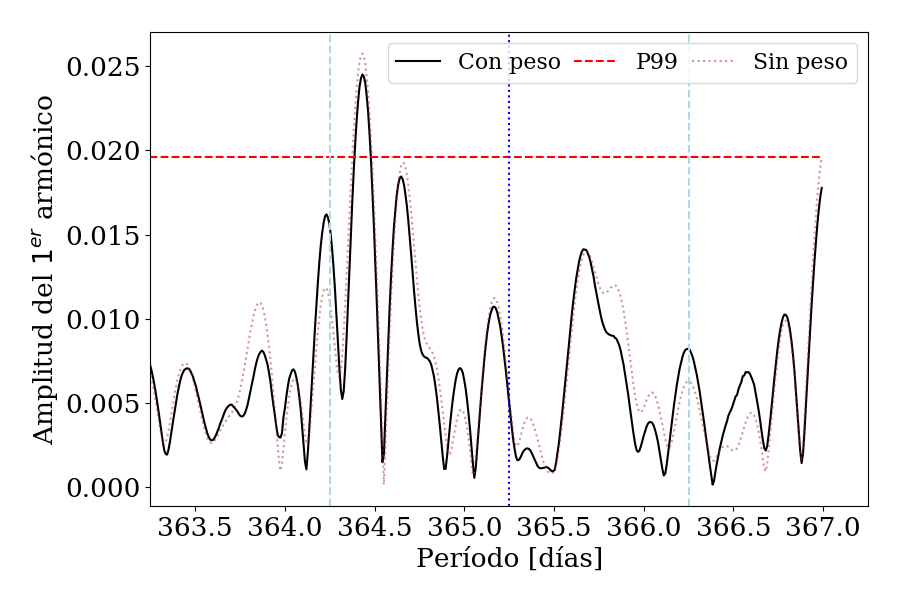
\includegraphics[width=0.5\textwidth]{Graficos/2019_Main_Array_4_8_EeV_con_vs_sin_peso.png}
	\caption{Disparos estándar: entre 4 EeV y 8 EeV, entre 2013-2019}
	\label{fig:48w}
\end{figure}
%fig

\subsubsection{Energía sobre 8\,EeV}

Para este caso utilizamos el archivo con el disparo estandar

\begin{figure}[H]
	\centering
	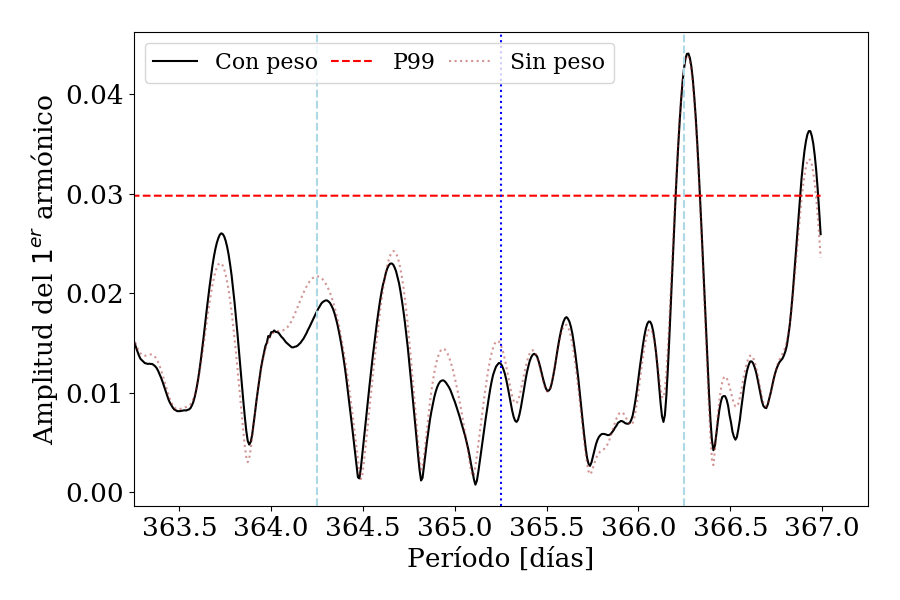
\includegraphics[width=0.5\textwidth]{Graficos/2019_Main_Array_8_EeV_con_vs_sin_peso.png}
	\caption{Disparos estándar: encima de 8 EeV, entre 2013-2019}
	\label{fig:8w}
\end{figure}
%fig




\subsection{Ampliando el rango de tiempo para el archivo del disparo estándar}

Amplié el rango de tiempo para poder compararlo con los gráficos anteriores, ya que se espera que mientras mayor sea el rango de tiempo los efectos espúreos disminuyen.

	\begin{table}[H]
	\centering
		\begin{tabular}{c|c|c|c}
	 		& UTC 			& Fecha		 	&  Hora GMT  \\ \hline
	Inicio	& 1104537600	&2005-01-01 	&00:00:00		\\
	Final 	& 1577825634	&2019-12-31 	&20:53:54		\\
		\end{tabular}
	\end{table}


\subsubsection{Energía entre 4\,EeV y 8\,EeV}

\begin{figure}[H]
	\centering
	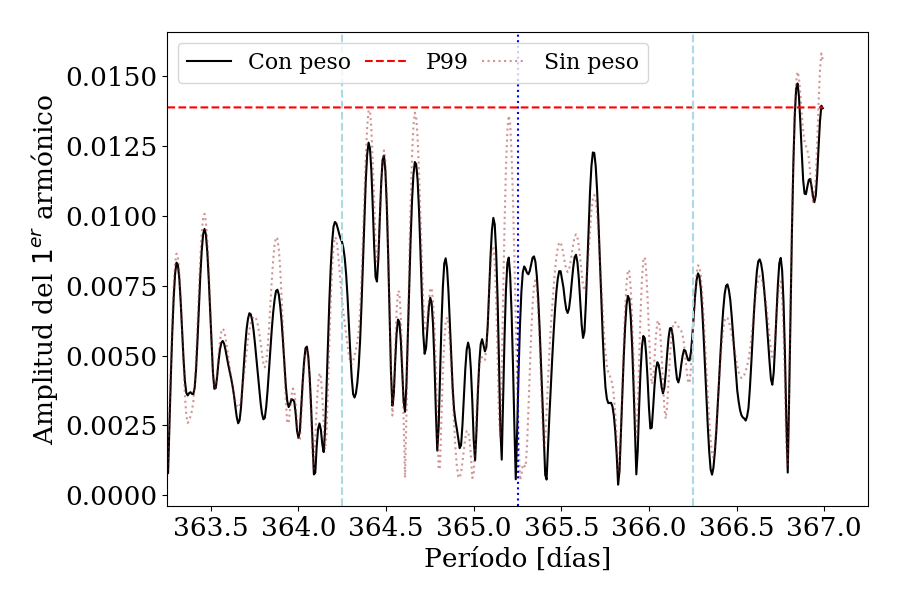
\includegraphics[width=0.5\textwidth]{Graficos/2019_Main_Array_4_8_EeV_con_vs_sin_peso_extended.png}
	\caption{Disparos estándar: entre 4 EeV y 8 EeV extendiendo el rango hasta el 2005}
	\label{fig:48w_extended}
\end{figure}
%fig

\subsubsection{Energía sobre 8\,EeV}


\begin{figure}[H]
	\centering
	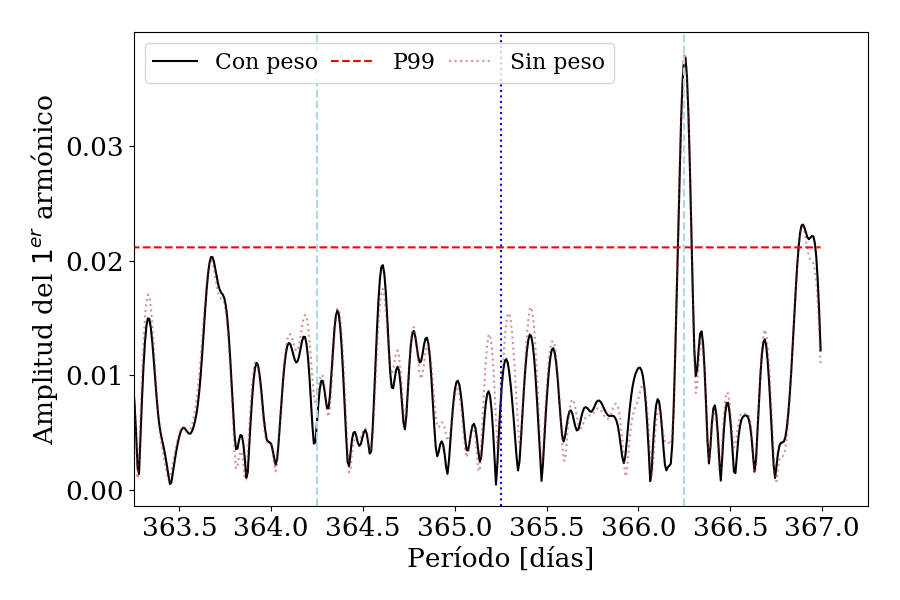
\includegraphics[width=0.5\textwidth]{Graficos/2019_Main_Array_8_EeV_con_vs_sin_peso_extended.png}
	\caption{Disparos estándar: encima de 8 EeV extendiendo el rango hasta el 2005}
	\label{fig:8w_extended}
\end{figure}
%fig


\end{document}
